%% V1.0
%% by Gabriel Garcia, gabrcg@gmail.com
%% This is a template for Udacity projects using IEEEtran.cls

%% Be Udacious!

\documentclass[10pt,journal,compsoc]{IEEEtran}

\usepackage[pdftex]{graphicx}
\usepackage{cite}
\usepackage{booktabs}
\usepackage{listings}
\lstset{basicstyle=\ttfamily,
  breaklines=true}
\usepackage{hyperref}
\hypersetup{
    colorlinks=true,
    linkcolor=blue,
    filecolor=magenta,
    urlcolor=cyan,
}
\usepackage{comment}
\hyphenation{op-tical net-works semi-conduc-tor}


\begin{document}

\title{RoboND: Map My World Project}

\author{Matthew Dewar}

\markboth{ROS, Mapping, SLAM, graphSLAM, RTAB-Map, Robotics Nanodegree Program, Udacity}%
{}
\IEEEtitleabstractindextext{%

\begin{abstract}
Simultaneous localization and mapping (SLAM) is a popular method of sensing and mapping a robots environment. For this project two simulated Gazebo environments will be mapped using RTAB-Map (Real-Time Appearance-Based Mapping) a graphSLAM approach using an appearance based method, in order to generate a 2D occupancy grid, as well an optimized RGBD 3d map gathered from an RGBD camera and a laser rangefinder mounted on a robot.
\end{abstract}

% Note that keywords are not normally used for peerreview papers.
\begin{IEEEkeywords}
Robot, IEEEtran, Udacity, \LaTeX, Localization.
\end{IEEEkeywords}}


\maketitle
\IEEEdisplaynontitleabstractindextext
\IEEEpeerreviewmaketitle
\section{Introduction}
\label{sec:introduction}

\IEEEPARstart{A}{n} effective robot must be able to navigate and interact with its environment by knowing where it is within its environment at any time. With an accurate map provided to the robot, the robot can localize itself within its environment to give a posterior probability of its pose within the given map. However in most real world cases the acquisition of a map prior to localization will not be possible. Under the assumption the robots poses are known and not noisy, a posterior map can be estimated using the occupancy grid mapping algorithm computing the log odds of the posterior belief. A grid of cells can be generated from this algorithm designating if the space is occupied, free, or unknown. In reality the robots pose will most likely be unknown which adds further complexity in that the robot must be able to simultaneously map and localize itself within its environment given unknown and noisy poses \cite{UdacityLesson15}. Numerous algorithms fittingly titled Simultaneous localization and mapping (SLAM) have been developed to solve this "chicken and the egg" problem.

In this report two simulated environments will be traversed by a rover equipt with a laser rangefinder and an RGBD camera using RTAB-Map (Real-Time Appearance-Based Mapping), which is a graphSLAM approach using an appearance based method involving loop closures. During loop closure, as the robot expands its known environment with images taken from its sensors, the new image is compared to each image within the robots memory \cite{UdacityLesson18}. If feature matches are found between images, loop closures are assigned between the two poses of these images and discrepancies in the graphSLAM map are resolved and optimized. Once the robot has traversed the entire map and at least three loop closures have been detected, an occupancy grid, and a appearance based 3d map will be generated.


\section{Background}
\label{sec:background}

SLAM algorithms can be broken up into categories that try and solve the Full SLAM, or the Online SLAM problem. The Online SLAM problem involves estimating the posterior only giving its current measurements and controls, whereas the Full SLAM problem involves computing the posterior over its entire path \cite{UdacityLesson17}. Popular techniques involving the Kalman filter or particle based filter approach fall into the online SLAM category, whereas continuous graphical approaches involving the full path history fall under the full SLAM problem. For this report the FastSLAM, and GraphSLAM algorithms will be investigated further, which both fall under the full SLAM problem.

\subsection{Occupancy Grid Mapping}
\label{subsec:occupancy}

With the assumption that the robot pose is known, occupancy grid mapping can be applied to estimate the posterior probability of a grid of cells determining the presence of an obstacle \cite{OccupancyWiki}. Utilizing the binary Bayes filtering algorithm the new state of each cell is calculated from the previous belief, the log odds ratio of probability of the posterior map given the measurements and the poses, and the log odds of the prior state of the map \cite{UdacityLesson16}. Through this algorithm a grid of cells estimating if the space is occupied, free, or unknown is generated.


\subsection{FastSLAM}
\label{subsec:fastslam}
FastSLAM first estimates the posterior of the robots trajectory by using a particle filter approach to solve the FullSLAM problem with known correspondences \cite{UdacityLesson17}. By using the particle approach the SLAM problem is now reduced to a mapping problem with known poses \cite{UdacityLesson17}.  Next, the posterior of the map is updated depending on whether the landmark has been observed or not by using a low dimensional extended kalman filter (EKF) modeled with a local Gaussian. FastSLAM is thus seen to be able to solve the Full SLAM problem by estimating the full robot path, as well as the online SLAM problem where each particle estimates the instantaneous pose of the robot \cite{UdacityLesson17}.

In order to solve the SLAM problem with FastSLAM in an arbitrary environment it must be combined with the occupancy grid mapping algorithm, modeling the environment with grid maps where each particle also maintains its own map. In the grid-based FastSLAM algorithm first the sampling motion is obtained estimating the current pose given the previous particle pose and current controls. Next the current map is estimated given the current measurements, the current particle pose, and the previous particle map. These first two steps can be solved by using the Mote Carlo Localization algorithm (MCL). In the last step, the likelihood of the current measurement is estimated given the current particle pose and the current particle map using the occupancy grid algorithm \cite{UdacityLesson17}.

\subsection{GraphSLAM}
\label{subsec:graphslam}
GraphSLAM solves the full SLAM problem covering the entire path and map, allowing the consideration and relationships between current and all previous poses \cite{UdacityLesson18}. GraphSLAM uses constraints to relate robot poses to its environment, where these constraints can be classified as either motion constraints, tying two poses together, or measurement constraints tying a measured feature to a pose. All of these constraints can be configured into a graph where the error is minimized over all the constraints using the Maximum Likelihood Estimation (MLE) principle. As the robot collects more and more sensory data from the environment around it a graph is constructed increasing with linear complexity over time. This graph is then optimized in the back end minimize the cost of the constraints. Any non linearity in the motion, or measurement constraints is linearized through the use of Jacobians in order to solve the system analytically. This process is iterated upon the previous solution until the solution converges. GraphSLAM is superior to the Fast SLAM algorithm in that it eliminates the chance in Grid-based FastSLAM where a particle will not be detected at a robots actual position.

For this report RTAB-Map (Real-Time Appearance-Based Mapping) will be used to generate occupancy grid maps, as well as the 3D appearance based map. RTAB-Map is  a graphSLAM approach using an appearance based method that uses data collected from vision sensors to localize the robot and construct a map of its environment. In RTAB-Map a process called loop closure is used to determine correspondence, with complexity increasing linearly as the map is expanded. RTAB-Map is optimized by using multiple strategies for loop closure to be done is real time. Obtaining an appearance based 3D map in addition to a 2d occupancy grid map, the robot can interact, and understand its environment more cohesively.

\section{Scene and robot configuration}
\label{sec:scene}

\subsection{Packages \& Robot Configuration}

Gazebo and RViz are utilized to manage the sensory input of the simulated environment through a Hokuyo laser range finder, and an Xbox kinect RGBD camera. The mobile rover consists of a base and two actuators on either side with odometry, with the range finder and camera mounted on the top and front of the robot respectively. The transformation tree of the robot is shown in Figure \ref{fig:tf-tree}. A program called rtabmap was wrapped in with ROS as a separate node used to perform SLAM on the environments. Rtabmap would take the sensor data, as well as the transform frame, and odometry data of the robot as inputs outputting a 3D appearance map, and 2D occupancy grid map localized with respect to the robot. A Teleop node was also added as the robot was user controlled, directed around Gazebo simulation in order to collect data. A list of these nodes and topics can be reviewed in Figure \ref{fig:rqtgraph}.

\begin{figure}[thpb]
      \centering
      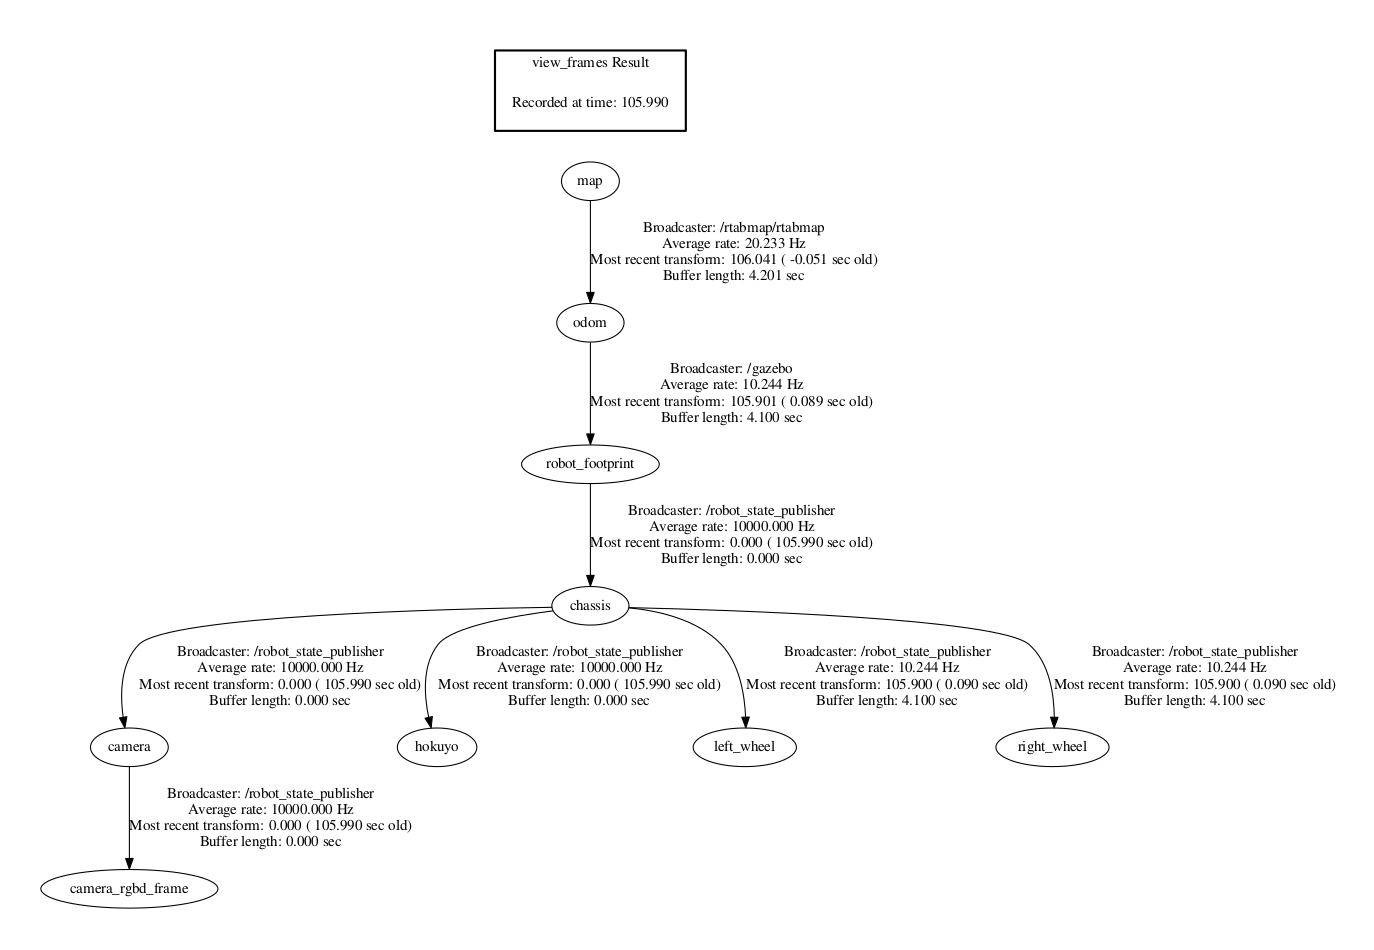
\includegraphics[width=\linewidth]{../img/frame.png}
      \caption{Transform frame tree of the Udacitybot fitted with a hokuyo lidar, and a kinect RGBD camera.}
      \label{fig:tf-tree}
\end{figure}

\begin{figure}[thpb]
      \centering
      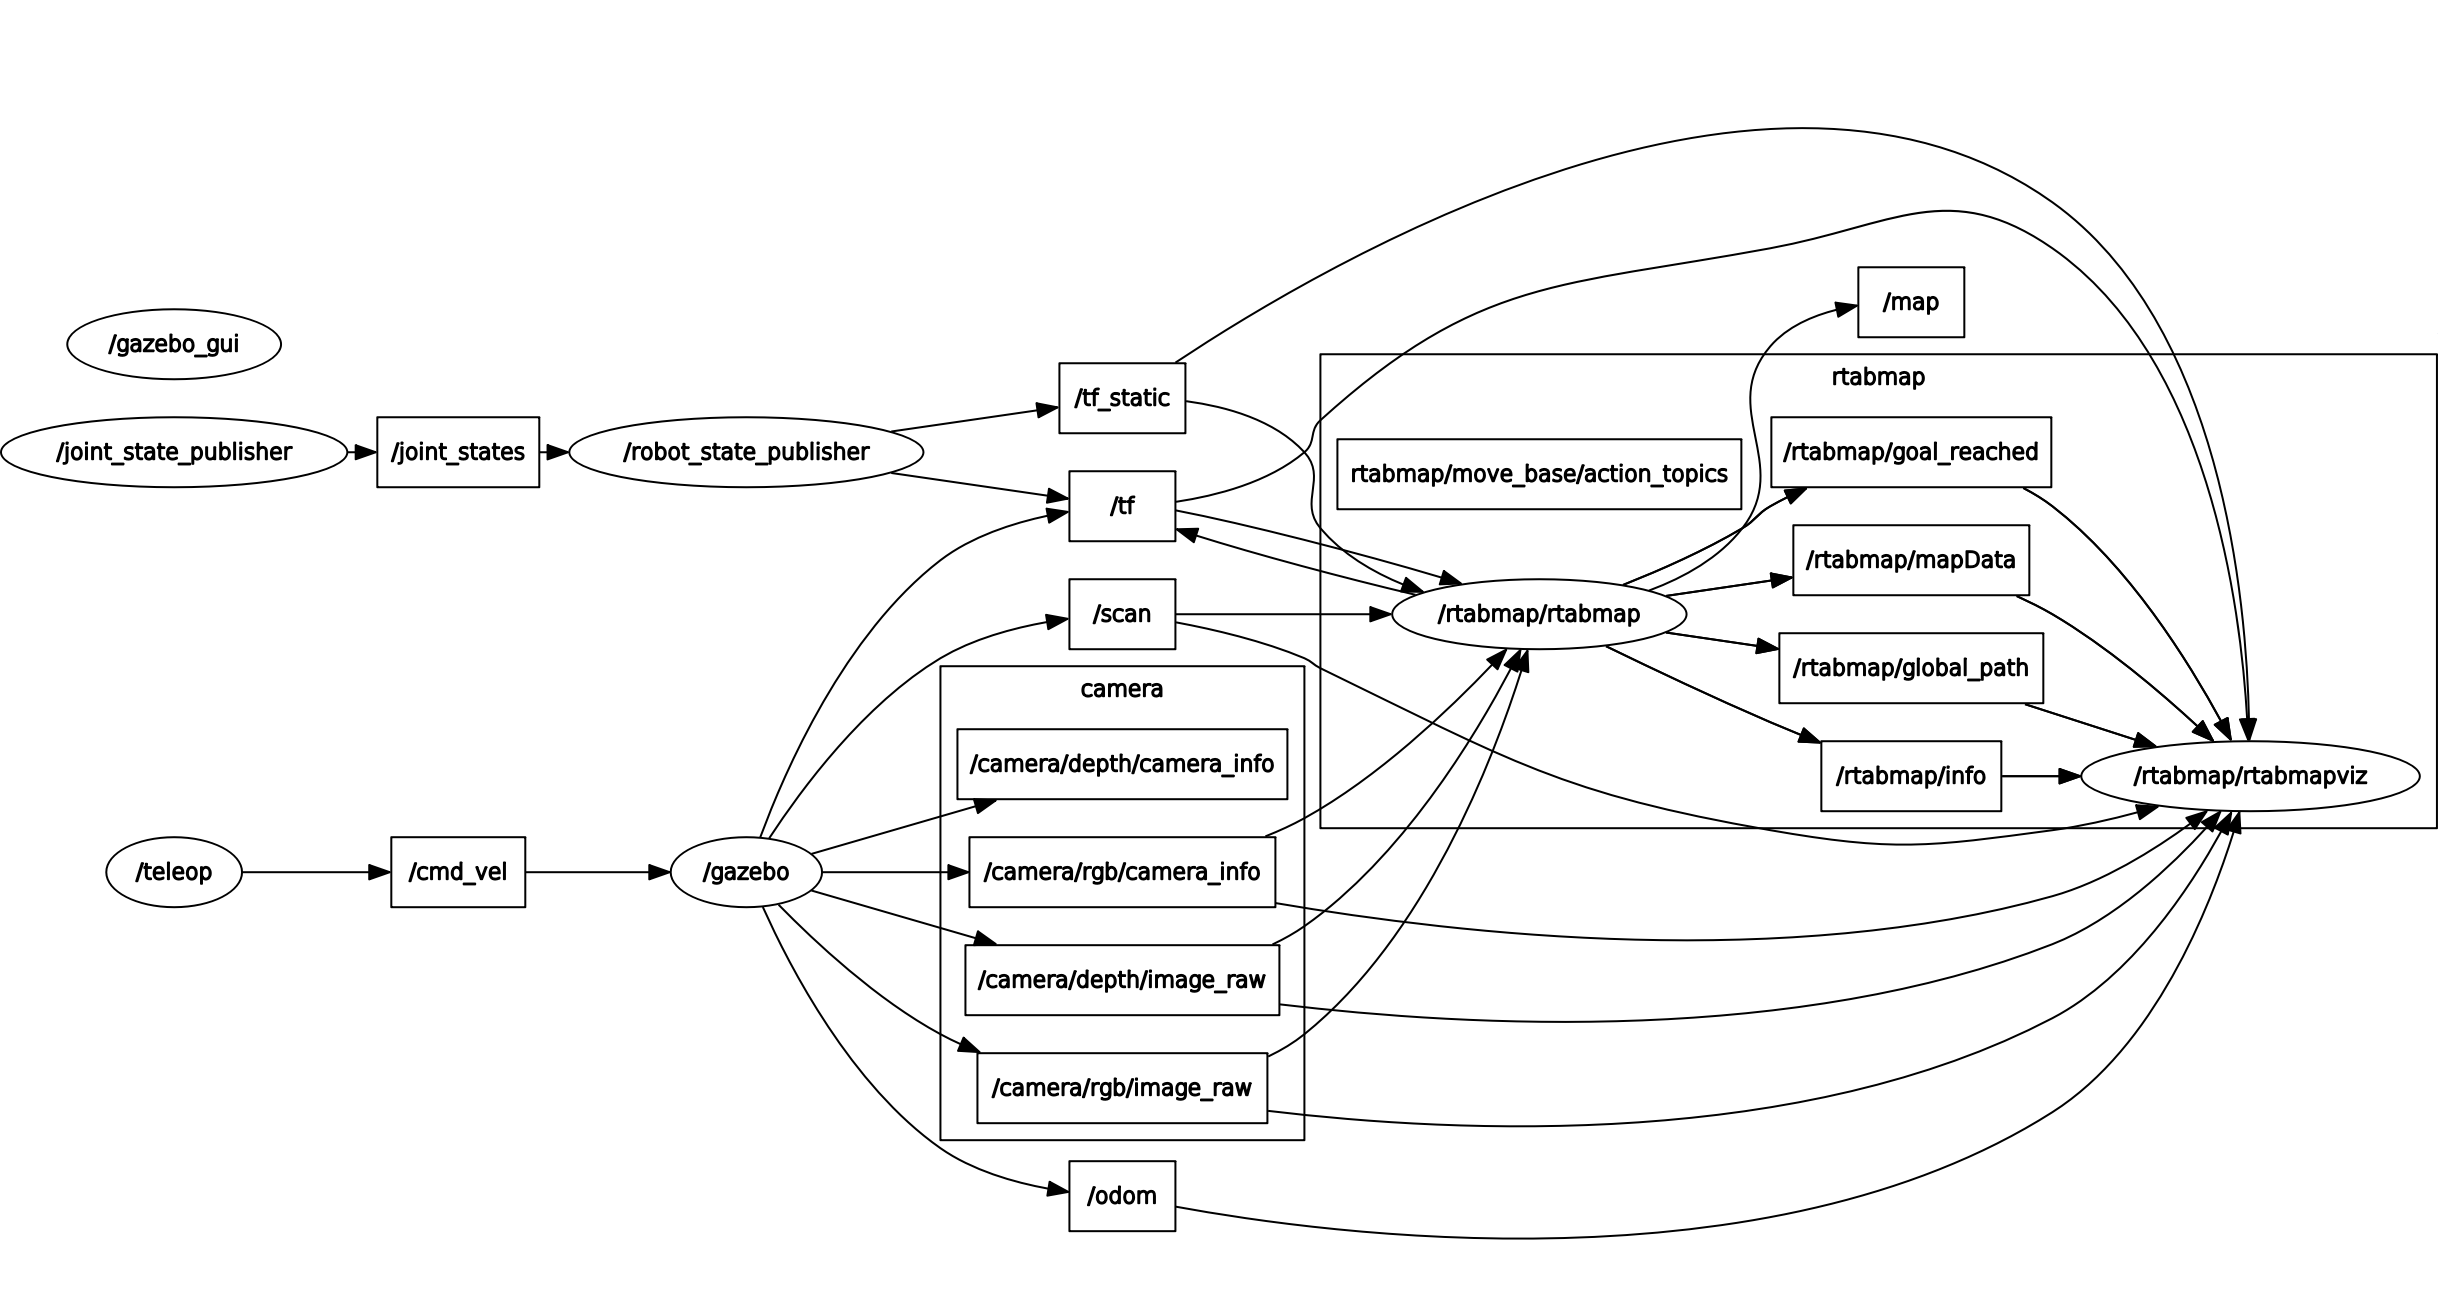
\includegraphics[width=\linewidth]{../img/rosgraph.png}
      \caption{ROS graph of node and topics used for the SLAM equipt robot.}
      \label{fig:rqtgraph}
\end{figure}


\subsection{worlds}

Mapping was performed in two simulated environments in Gazebo. The supplied environment from Udacity consisted of a kitchen and dining room and can be found in the kitchen\_dining.world file of this reports repository. The custom environment used for this project was taken from the 3DGEMS online dataset \cite{3DGems}, which was a large office space filled with chairs, tables, office desks/supplies, and lunch facilities. This office world can be located in the office\_env\_large.world file of this reports repository. Both the kitchen and office Gazebo environments are shown in Figure. \ref{fig:gazebokitchen}, and Figure. \ref{fig:gazebooffice} respectively.

\begin{figure}[thpb]
      \centering
      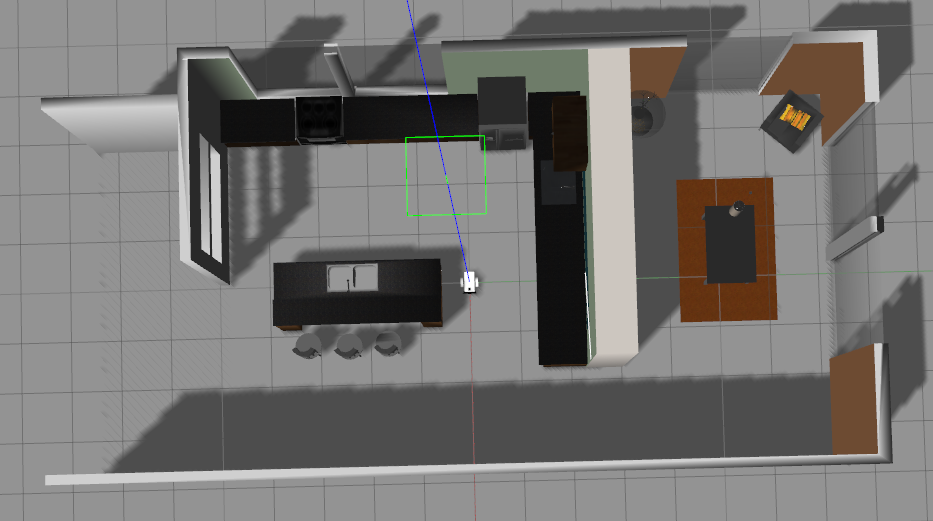
\includegraphics[width=\linewidth]{../img/gazebo_kitchen.png}
      \caption{Provided simulated environment for mapping.}
      \label{fig:gazebokitchen}
\end{figure}

\begin{figure}[thpb]
      \centering
      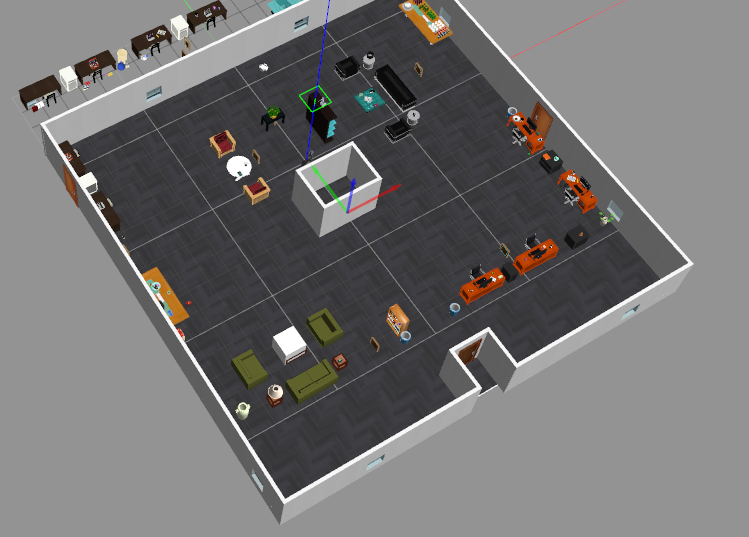
\includegraphics[width=\linewidth]{../img/gazebo_office.png}
      \caption{Person simulated environment of an open office concept. Models and world were taken from 3DGEMS \cite{3DGems}}
      \label{fig:gazebooffice}
\end{figure}


\section{Results}
\label{sec:results}


\subsection{Provided Gazebo World}
\label{subsec:kitchenworld}

After teleoperating several path laps with the robot around each environment maps of both 2D occupancy grid maps and 3d maps were constructed each containing over three loop closures. For the kitchen world the loop closures and the path odometry can be seen in Figure. \ref{fig:loopclosureKitchen}, with the output occupancy grid map, and 3D map displayed in Figure. \ref{fig:occupancyKitchen}, and Figure. \ref{fig:3DKitchen} respectively.

\begin{figure}[thpb]
      \centering
      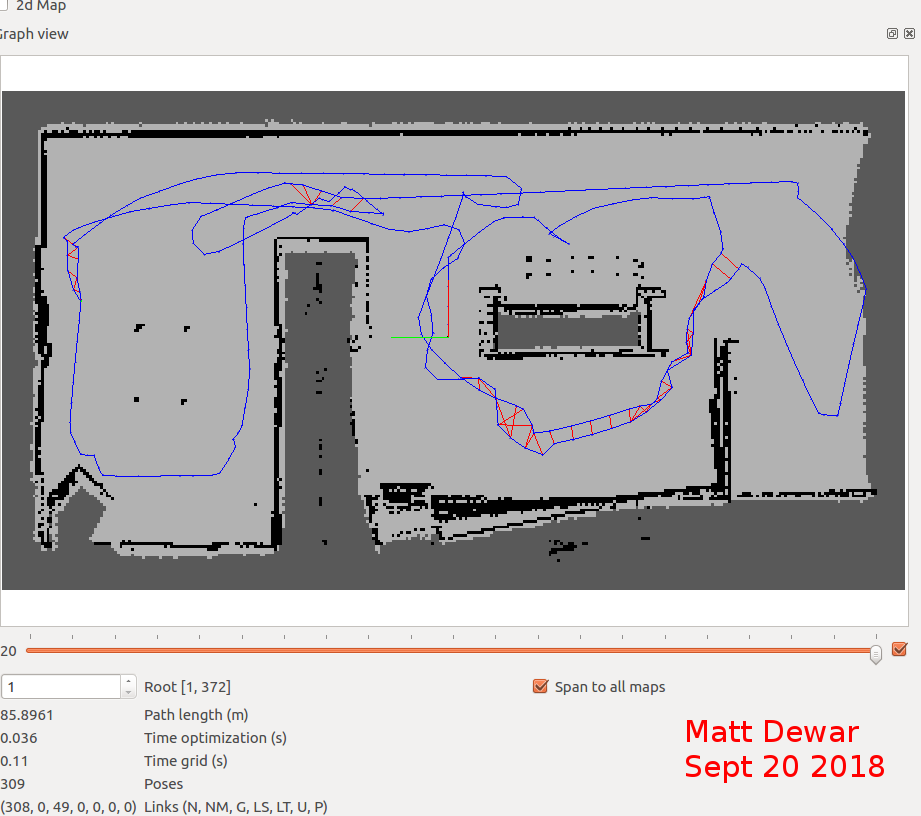
\includegraphics[width=\linewidth]{../img/loop_closure_kitchen2.png}
      \caption{Loop closures and robot path taken in kitchen world to generate map using RTAB-Map}
      \label{fig:loopclosureKitchen}
\end{figure}

\begin{figure}[thpb]
      \centering
      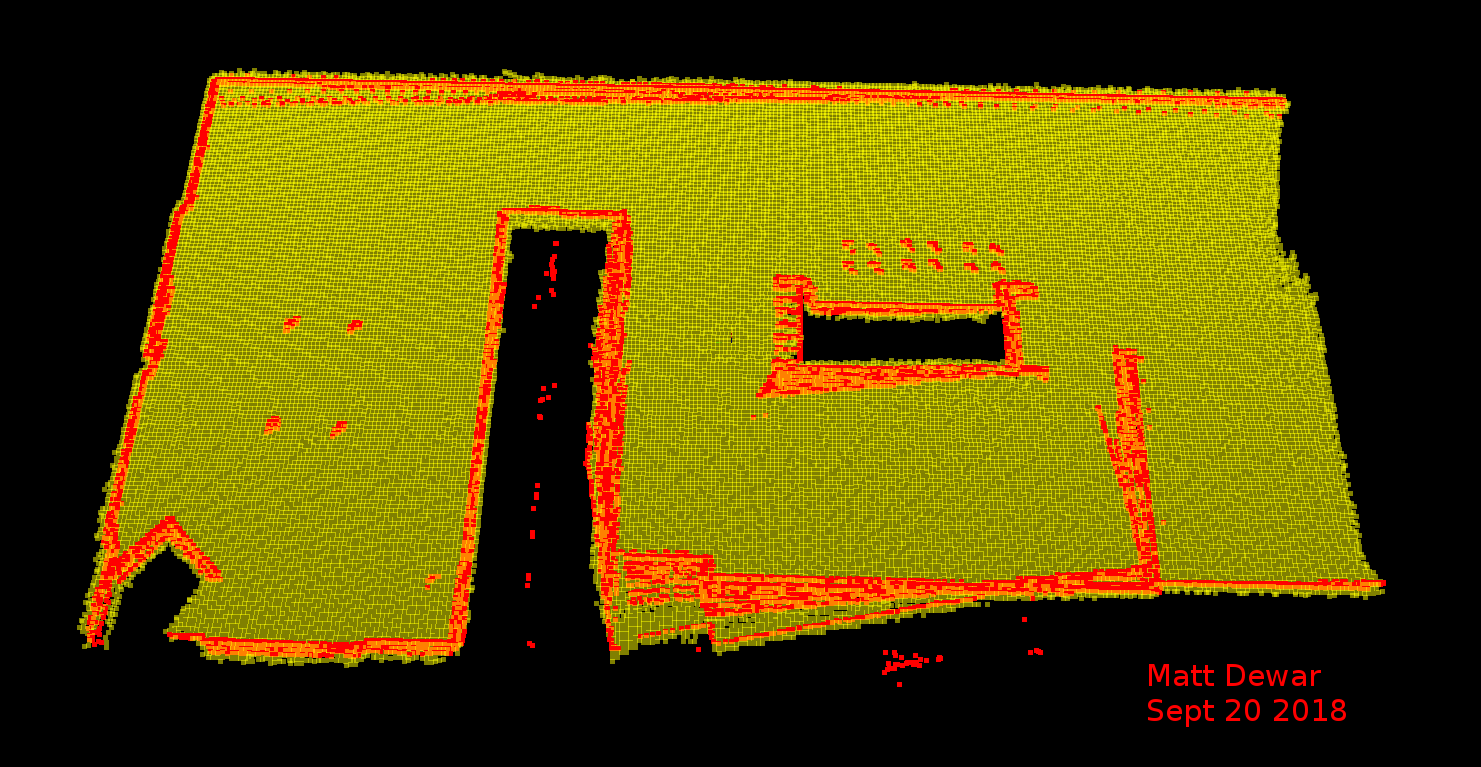
\includegraphics[width=\linewidth]{../img/kitchen_occupancy_map.png}
      \caption{Occupancy grid map of the kitchen world, where red is occupied space, and yellow is free space, and black is the unknown space.}
      \label{fig:occupancyKitchen}
\end{figure}

\begin{figure}[thpb]
      \centering
      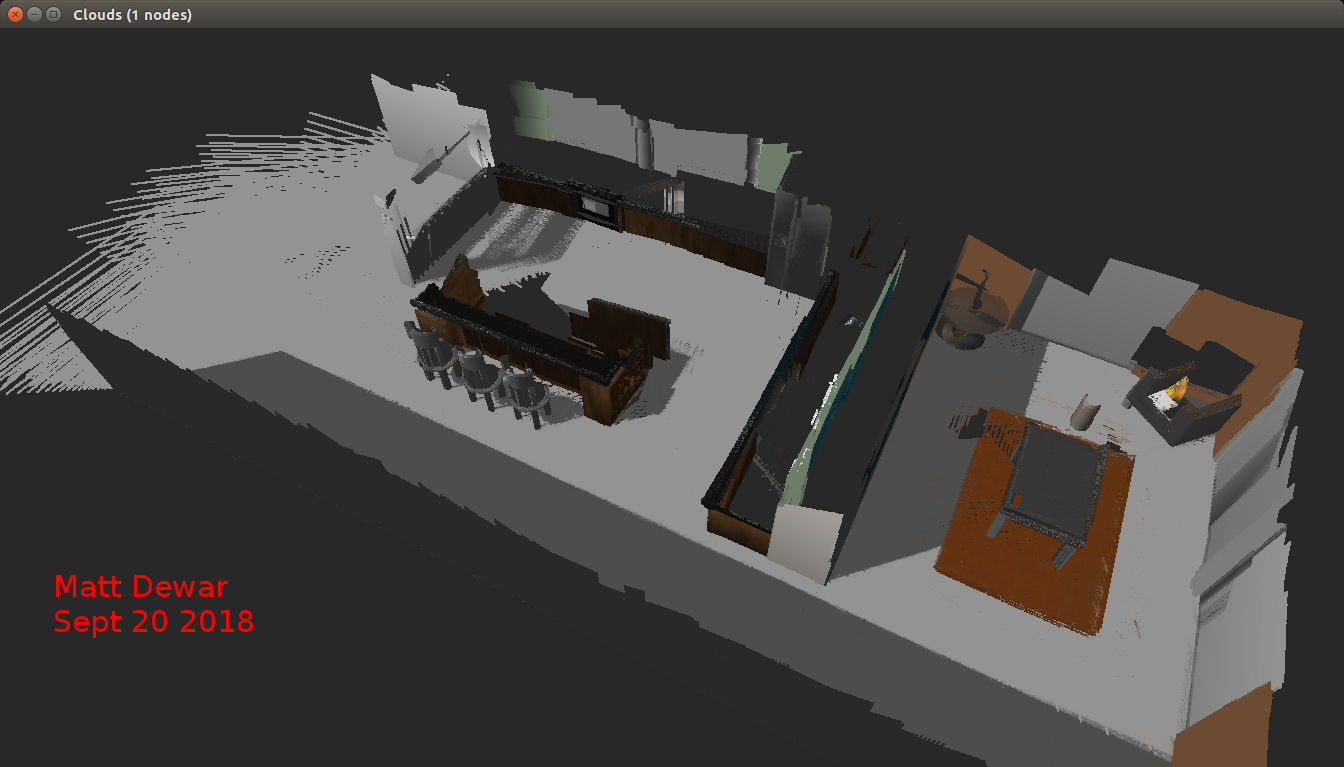
\includegraphics[width=\linewidth]{../img/3d_map_kitchen.png}
      \caption{3D map of the kitchen world generated with the RTAB-Map database viewer.}
      \label{fig:3DKitchen}
\end{figure}

\subsection{Personal Gazebo World}
\label{subsec:officeworld}

For the Office world, loop closures, the 2D occupancy grid map, and 3D map are shown in Figures. \ref{fig:loopclosureOffice}-\ref{fig:3DOffice}, where the occupancy grid is identifiable, and the 3D map of the environment is clearly recognizable.

\begin{figure}[thpb]
      \centering
      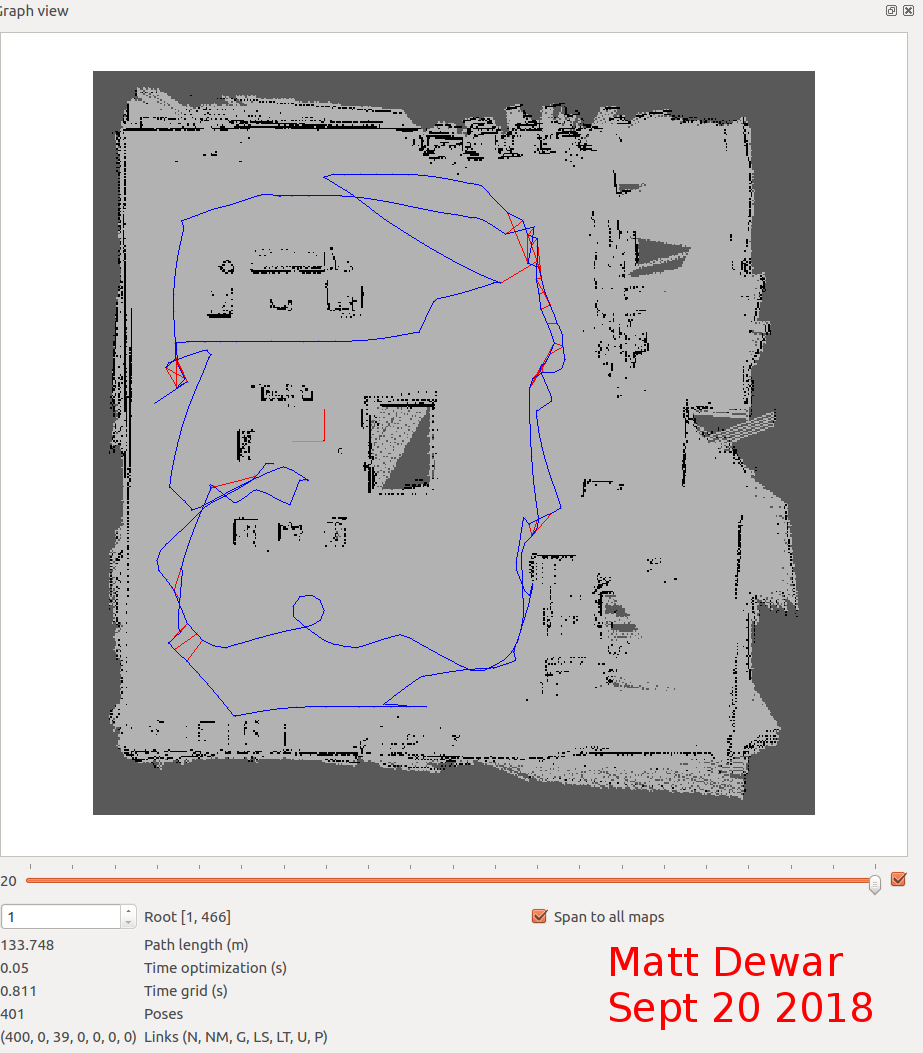
\includegraphics[width=\linewidth]{../img/loop_closure_office2.png}
      \caption{Loop closures and robot path taken in office world to generate map using RTAB-Map}
      \label{fig:loopclosureOffice}
\end{figure}

\begin{figure}[thpb]
      \centering
      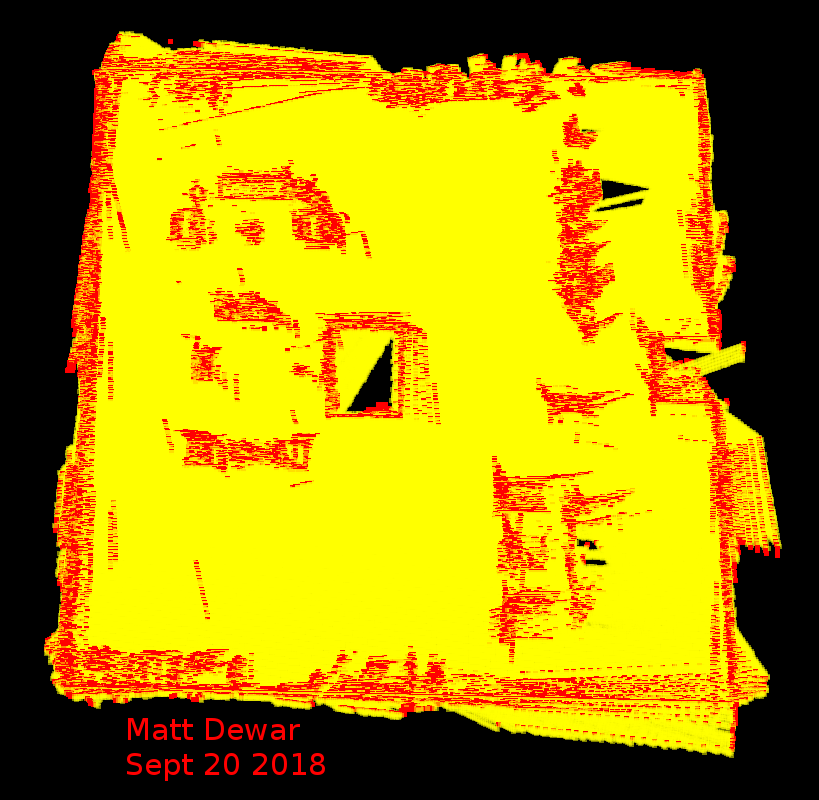
\includegraphics[width=\linewidth]{../img/office_occupancy_map.png}
      \caption{Occupancy grid map of the office world, where red is occupied space, and yellow is free space, and black is the unknown space.}
      \label{fig:occupancyOffice}
\end{figure}

\begin{figure}[thpb]
      \centering
      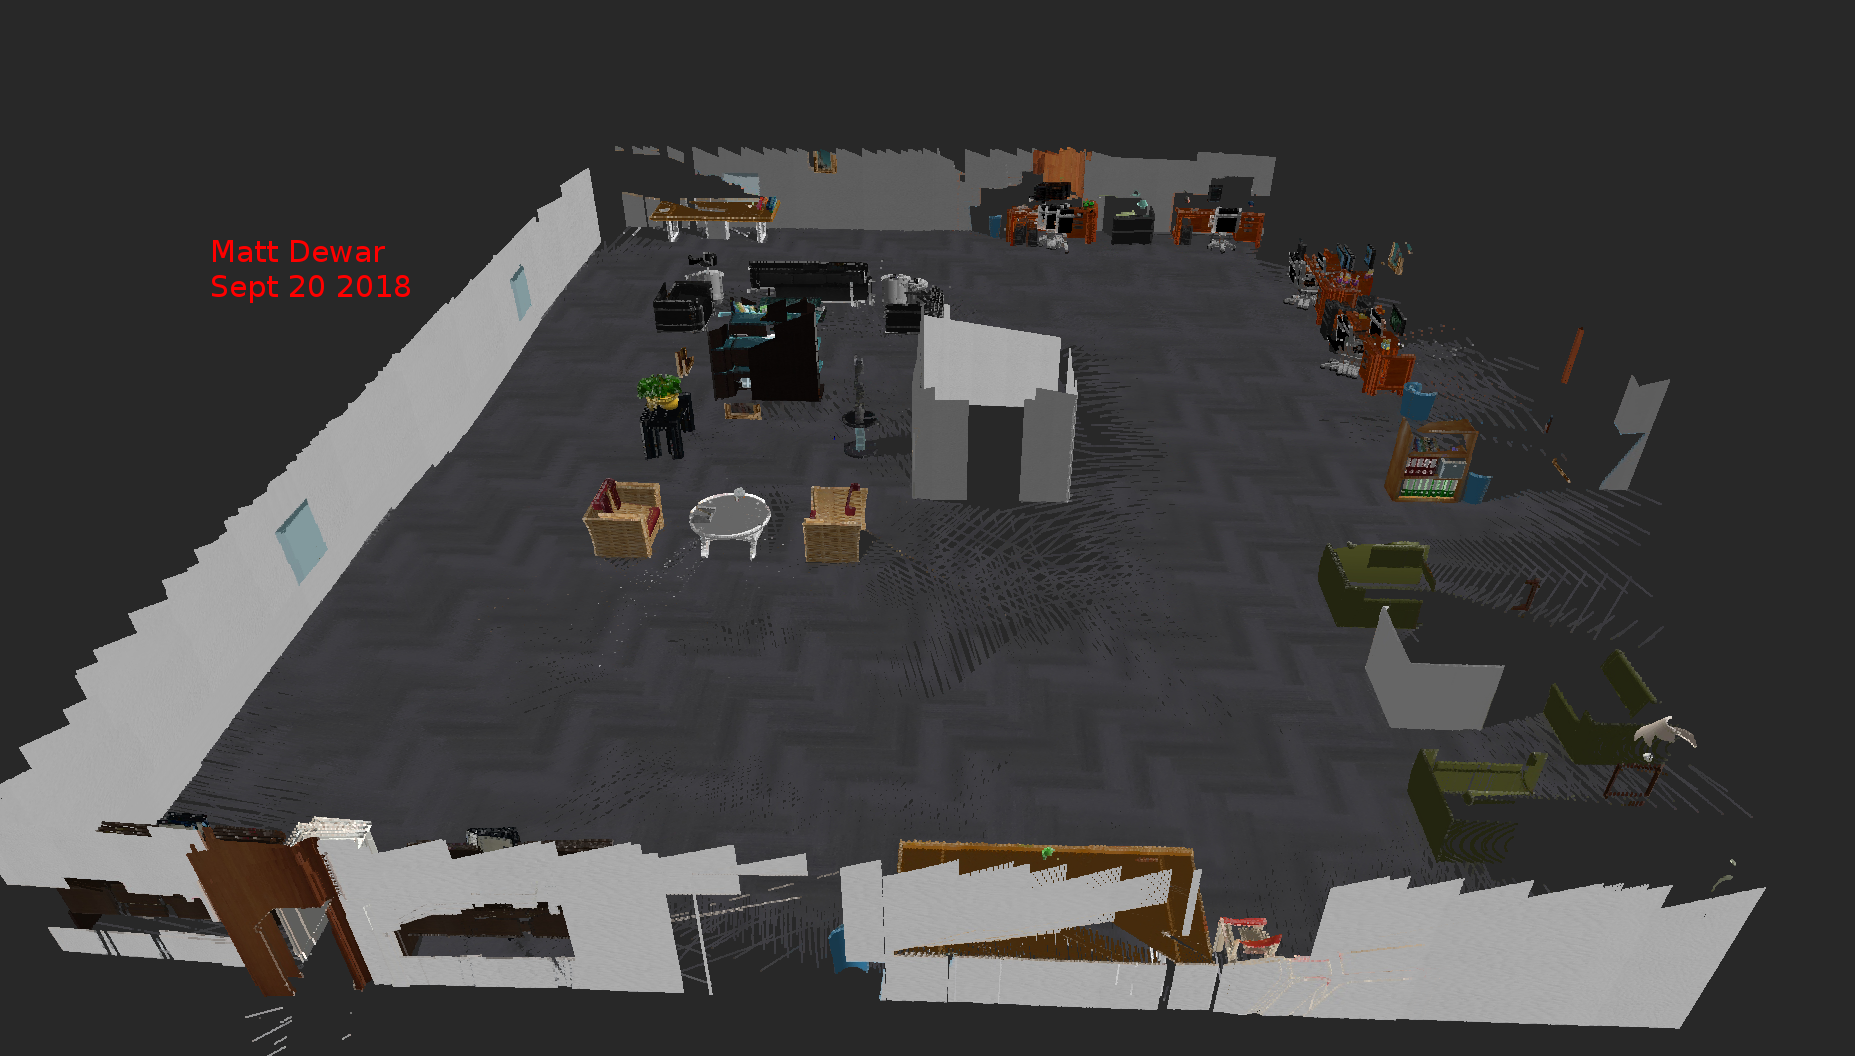
\includegraphics[width=\linewidth]{../img/3d_map_office.png}
      \caption{3D map of the office world generated with the RTAB-Map database viewer.}
      \label{fig:3DOffice}
\end{figure}


\section{Discussion}
\label{sec:discussion}
Overall, RTAB-Map was successful in generating 2D occupancy grid maps, as well as 3D appearance based maps for each of the Gazebo environments. RTAB-Map was also successful in measuring correspondence, effectively extracting features from images and compiling visual bag-of-words for each image, retrieving appropriate candidates from its Long-term memory for loop closure detection. A few different runs of the kitchen world were performed, both zigzagging and re-tracing paths for a large number of loop closure detections, and only running through each section once or twice with loop closures on the connecting pieces. It was found that the best occupancy grids appear to be generated with less loop closures, even after graph optimization. However, the optimization features were not experimented with to any great extent for this report. Comparing the Office world to the kitchen world we can see that the occupancy grid is a lot less uncertain in the office world. This maybe due to the larger environment that the robot is required to map, or the repetitive or nondescript objects in the environment causing false loop closures. In the 3D map for the office, errors in object resolution, or objects 'blurring' were much higher than in the kitchen environment for potentially the same reasons. Loop closures where better detected by rotating the robot around in place rather than just trying to retrace a previous lap done by the robot.


\section{Conclusion / Future work}
\label{sec:conclusion}

In conclusion, 2D occupancy gird maps, and 3D appearance point cloud maps were generated for both simulated office and kitchen environments using the RTAB-Map library. Further work needs to be done in order to generate the maps by automating the robots discovery path via waypoints, or a sensory algorithm to move around its unknown environment without being teleoperated. The Author also needs to experiment with graph optimization features (TORO, G2O, or GTSAM) found in RTAB-Map to try and refine the output maps. The next step would be to apply RTAB-Map to a real world environment such as a home or office using the Jetson TX2 platform.


\bibliography{bib}
\bibliographystyle{ieeetr}

\end{document}
